\section{Evaluation} %FIXME improvee!!!
Case Study: (find a good ones) FP Project

[INSERT EXAMPLES HERE]
\begin{lstlisting}[basicstyle=\ttfamily, caption="Sample code"]
  (if (>= n_jogadas 35)
        #T
        #F)
\end{lstlisting}

\begin{figure}
\centering
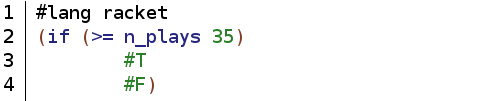
\includegraphics[width=\linewidth]{images/example1.png}
\label{exampleIfTrueFalse}
%\caption{Information flow between modules.}
\end{figure}

\begin{figure}
\centering
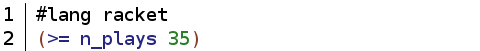
\includegraphics[width=\linewidth]{images/transformation1.png}
\label{exampleIfTrueFalse}
%\caption{Information flow between modules.}
\end{figure}

\begin{figure}
\centering
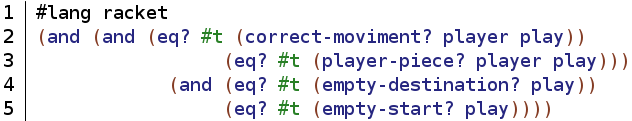
\includegraphics[width=\linewidth]{images/example2.png}
\label{exampleIfTrueFalse}
%\caption{Information flow between modules.}
\end{figure}

\begin{figure}
\centering
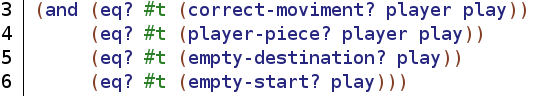
\includegraphics[width=\linewidth]{images/transformation2.png}
\label{exampleIfTrueFalse}
%\caption{Information flow between modules.}
\end{figure}

\begin{lstlisting}[basicstyle=\ttfamily, caption="Refactoring and expression"]
(and
  (and
   (eq? #t (movimento-valido? jogador jogada))
   (eq? #t (peca-jogador? jogador jogada)))
  (and
   (eq? #t (casa-destino-vazia? jogada))
   (eq? #t (casa-inicial-vazia? jogada))))
\end{lstlisting}


These are some real examples of pieces of code made for beginners, in the course
project of the programming introductory course.



The examples show the usage of some of the refactoring operations previous presented
and here is explained the motivation for their existence.
This examples appear repeatedly in almost every project supporting the need to
this kind of refactoring.

Beginners often use error and trial approach in code writing which led %FIXME
to peaces of code like the presented above.
If the users had a refactoring tool that highlighted their code in areas that
could be improved, they probably would not have this kind of code.


\section{Conclusion}

%growing importance of programing.
%growing importance support tools for beginners
%lack of refactoring tools for beginners
%the use that the beginners might use


The growing interest in programming as a skill combined with the need of areas
non related with any computation field creating the need to improve the support
given to the beginner user. %FIXME
Therefore a refactoring tool designed for beginners in a pedagogical environment such as DrRacket %FIXME IMPROVE
 would benefit those users as it would help them in their first contact with a
 refactoring tool and improve their code safely. %suggest the refactorings?
%this combined/composition with the importance increase of programming

Our solution tries to help those users to improve their programs and to facilitate
the first contact with a refactoring tool.
By having a refactoring tool designed for beginners in a pedagogical environment
that suggests possible refactoring operations.

We also shown the practicability of the refactoring tool with simple refactoring operations
that improved safely the beginners code.

%The second one is the crescent importance of the support given to beginner users %FIXME
%that made JetBrains, a company known for their professional IDEs, to make PyCharm - edu
% an IDE that is aimed for beginners and it also has incorporated a refactoring tool.
%Lastly the refactoring tools concern with professionals leaves the beginner
% user helpless.
% A refactoring tool aimed for beginners would help them to safely improve %FIXME!!!!!
% their code while giving those users the first contact with a refactoring tool.

%\section{Future work}
There are some improvements that we consider important and in the future it would  %FIXME
be a huge improvement detecting when a developer is refactoring in order to help the developer finish the
refactoring by doing it automatically \cite{ge2012reconciling}.
%This would be important specially for beginners that would help them finishing
%the transformations safely while teaching them refactoring operations. %FIXME yup...

%Our automatic detecting of duplicated code is still very naive.
The detection of duplicated code is still very naive and improving to understand if
two variables represent the same even if the names are different or even if the
 order of some commutative expressions is not the same would make a huge improvement
 on the automatic suggestion.

%Because the goal of the refactoring tool is to let beginners have the first touch
%with refactoring tools, having a good preview is important to show the user what
%the refactoring operation does.
%Improving the existing preview and changing from the menu to the code directly
%would be a great improvement to this refactoring tool.

%Improve the Preview of the refactoring operations.

%Improving automatic detection %TODO add code smells
It is possible to improve the automatic suggestion of refactoring operations by
having different colors for different types of refactoring operations.
This would let the user know what refactoring is being suggested without having to
select the area.
Another improvement that could be made is the color intensity of the suggestion.
With a lower intensity for low "priority" refactoring operations and a high intensity
for higher "priority". Thus giving the user a better knowledge of what is a better
way to solve a problem or what is a strongly recommendation to change the code.
